\namedsection{Aufbau eines Konnektors}{T}
Wie zuvor in Kapitel \ref{chap:Technologieauswertung} erwähnt, hatten wir uns nach sorgfältiger Evaluierung für eine Implementierung mit Java und dem Spring Boot Framework entschieden. Da das Spring Boot Framework einen opinionated Ansatz\footnote{https://www.baeldung.com/spring-vs-spring-boot} für die Implementierung verfolgt, besteht unser Konnektor aus dem Presentation Layer, Business Layer und dem Persistence Layer. Unsere APIs wurden dabei in den Controller-Klassen im Presentation Layer implementiert, die nach Aufruf unsere Service-Klassen nutzen, um Geschäftslogik durchzuführen. Je nachdem, welche Aktionen ausgeführt werden soll, rufen sie entsprechende Spring Beans\footnote{Siehe https://www.baeldung.com/spring-bean} auf, um gewisse Funktionen durchzuführen. Dies können Mapper-Beans sein, um Plain Old Java Objects (POJOs)\footnote{Siehe \\ http://openbook.rheinwerk-verlag.de/javainsel9/javainsel\_10\_003.htm\#mj37a114845c2154c378d52ab696e22192} zu mappen oder QuartzJob-Beans, um Job Schedules auszuführen. Für die Durchführung der Spring Batch Jobs werden JobLauncher-Beans verwendet, die dann in der Lage sind, die entsprechenden Batch Jobs durchzuführen. Sobald Aktionen gegen die Datenbank durchgeführt werden sollen, werden Repository/Mapper Interfaces verwendet, die als Abstraktionsschicht dienen und entweder MyBatis für die MSSQL-Datenbank oder die MongoDB-API verwenden, um die entsprechenden Datenbankoperationen auszuführen. Die Abbildung \ref{fig:Aufbau eines Konnektors} veranschaulicht den Aufbau eines Konnektors.

\begin{figure}[!h]
\centering
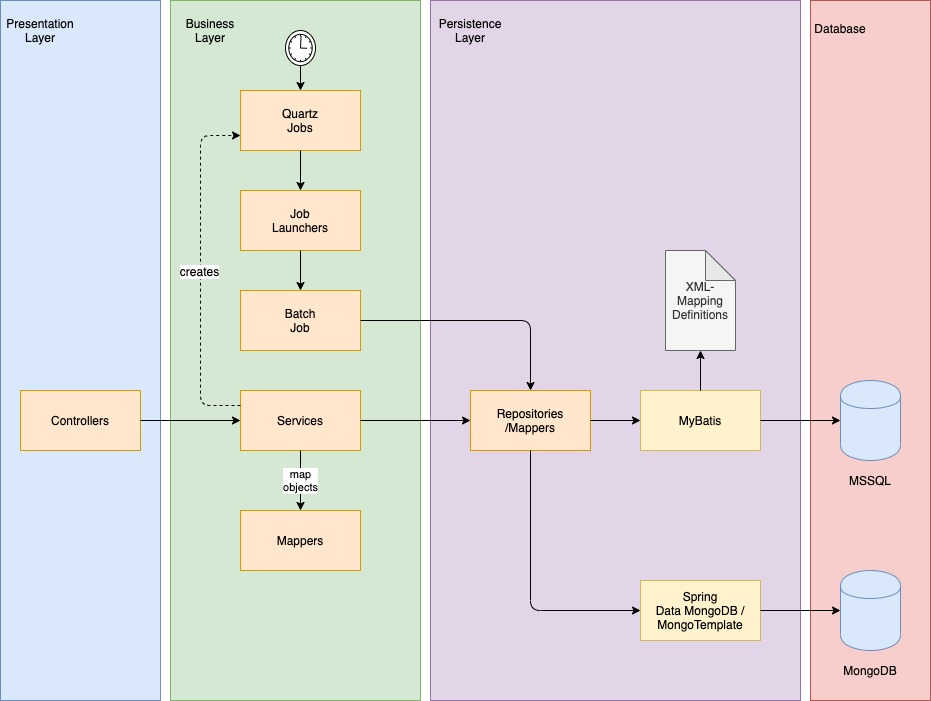
\includegraphics[width=15cm]{images/00_software_architecture/02_connector_structure/connector_structure.jpg}
\caption{Aufbau eines Konnektors}
\label{fig:Aufbau eines Konnektors}
\end{figure}